\chapter{Stationary properties} 
\label{chap:stationary}
\label{chap:stationary_properties}
The stationary properties of the system are defined by its spectrum. In this chapter an effective boundary condition for long-wave wave functions is introduced, wavefunctions are obtained, subgap states are found and  and the stationary supercurrent is investigated.

\section{Boundary condition}

To obtain the spectrum of the system it's necessary to find the wavefunctions inside the barrier. As the barrier chemical potential  is the biggest energy parameter of the problem, they are defined by the Hamiltonian:
\begin{gather}
\label{barrier_Hamiltonian}
	H(y)
	=
	\br{
		\frac{p^2}{2m}
		+\mu_b
	}\tau_z,  ~~~~~~~~~-\frac{L}{2}<y<\frac{L}{2}.
\end{gather} 

As low energies are the under consideration, in Schroedinger equation the energy term can be omitted, so $ p_b\approx\pm i \sqrt{2m\mu_b} $. Matching the wavefunctions and their derivatives inside and outside the barrier, we take barrier wavefunctions out of the problem and obtain the following boundary condition for wavefunctions on the left and on the right of the barrier:
\begin{gather}
\label{bc_initial}
	\begin{cases}
	\psi_L + b\partial_y\psi_L=t(\psi_R + b\partial_y\psi_R) \\
	\psi_R - b\partial_y\psi_R=t(\psi_L - b\partial_y\psi_L)
	\end{cases}
\end{gather}

where $ \psi_{L,R}=\psi\br{\mp\frac{L}{2}} $, $ b=\br{{2m\mu_b}}^{-\frac{1}{2}}=\frac{1}{p_b} $ --- the penetration depth for the particle inside the barrier and $ t = e^{-\frac{L}{b} }$ --- the tunneling constant assumed to be small: $ t\ll 1 $. This condition means, that the size of the barrier $ L $ should be  much bigger that the penetration depth $ b $.

The condition (\ref{bc_initial}) is invariant under the combined action $ L\leftrightarrow R $, $ y\to-y $. To simplify further analysis we reverse the direction in the left wire and shift both ends of the wires from $ y= \frac{L}{2} $ to $ y=0 $. The boundary condition than becomes:
\begin{gather}
\label{bc_transformed}
\begin{cases}
\psi_L - b\partial_y\psi_L=t(\psi_R + b\partial_y\psi_R) \\
\psi_R - b\partial_y\psi_R=t(\psi_L + b\partial_y\psi_L)
\end{cases}
\end{gather}
This transformation is illustrated on fig. \ref{fig:bctransform}. Note

The boundary condition (\ref{bc_transformed}) can be rewritten with the spinor $ \Psi=\br{\psi_L, \psi_R}^T $ and Pauli matrices $ \hat{s}_i $ in LR space:
\begin{gather}
	\br{1-t\hat{s}_x}\Psi-\br{1+t \hat{s}_x}b\pdy\psi=0
\end{gather}
Since for all $ t\ne 1 $ (recall, that $ t\ll1 $) the matrix is $ 1\pm t\hat{s}_x $ in invertible multiplying the last equation by $ \br{1-t\hat{s}_x}/\br{1+t^2} $ yields:
\begin{gather}
\label{bc_LR_space}
	\br{1-2\tilde{t}\hat{s}_z-\tilde{b}\pdy}\Psi=0
\end{gather}
where $ \tilde{t}=\frac{t}{1+t^2} $, $ \tilde{b} = \frac{1-t^2}{1+t^2}b $. In the leading order in $ t $, which corresponds to the tunneling limit, $ \tilde{t}=t $, $ \tilde{b} = b $.
\begin{figure}[H]
	\centering
	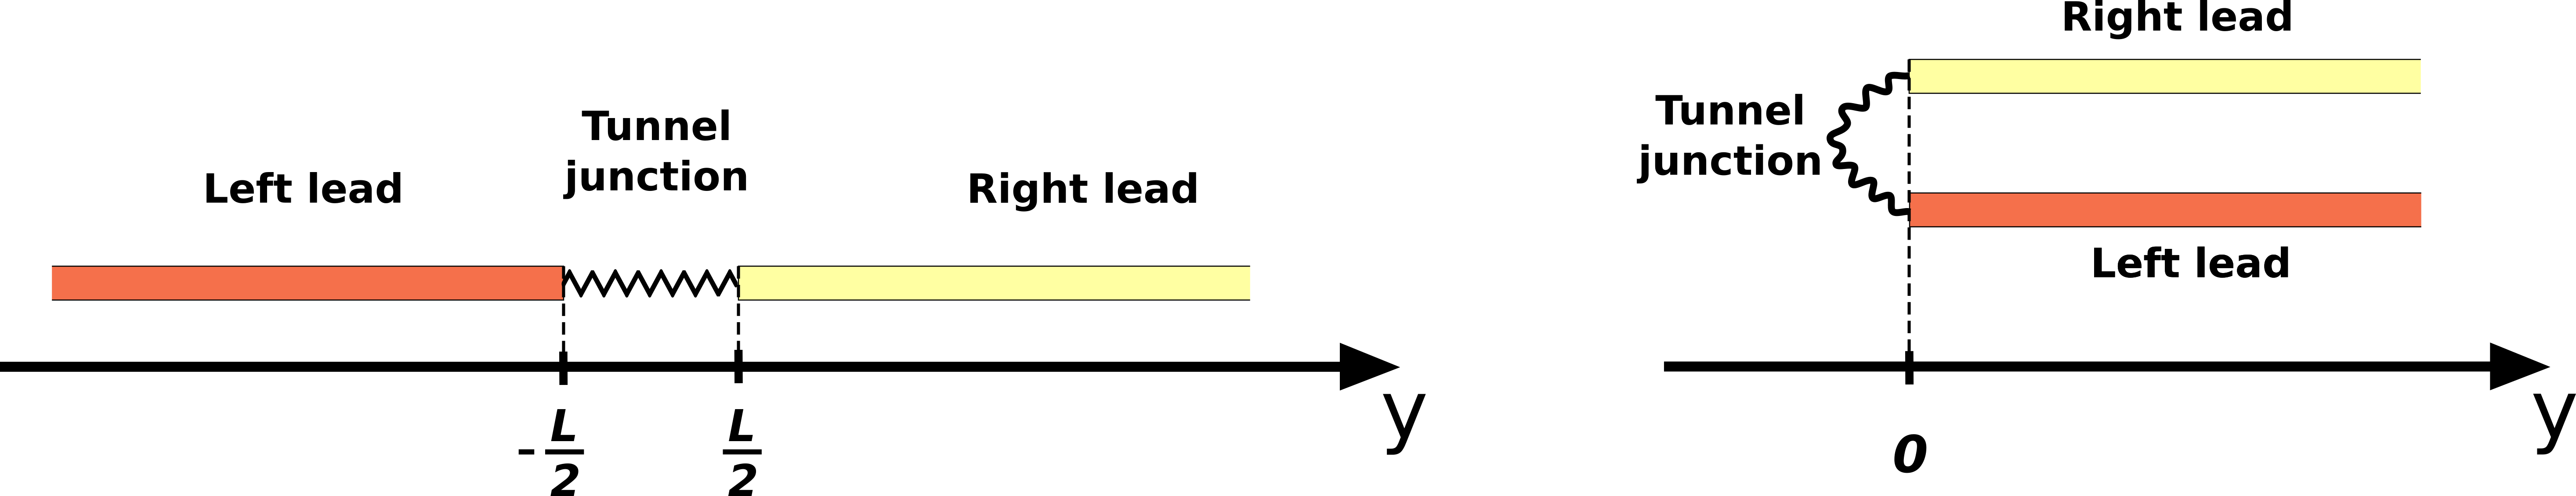
\includegraphics[width=0.9\linewidth]{images/bc_transform}
	\caption{Illustration of switching the direction of left wire}
	\label{fig:bctransform}
\end{figure}

One can argue that in tunneling limit the second and the third term in (\ref{bc_LR_space}) are much smaller than the first one and should not be taken when the leading order is considered. However, if the second term is omitted, the wires become disconnected, and no tunnel effects can be found. The same is true for the third term --- if it's not present, the boundary condition immediately implies $ \Psi\br{0} = 0 $, so the wires become disconnected again.

\section{Short-wave wavefunctions}  
\label{sec:short-wave_wavefunctions}
As was pointed in section \ref{sec:high_and_low_modes}, the short-wave wavefunctions should be described with the Hamiltonian (\ref{short-long_hamiltonian}) with a superconducting term:
\begin{gather}
\label{high_mods_hamiltonian}
	H=\br{\frac{p^2}{2m}-up\hat{s}_z\sigma_z}\tau_z+\Delta\tau_\phi
\end{gather}
here the multiplier $ \hat{s}_z $ is added in the spin-orbit coupling term, as the direction of the left wire is inverted, so to write a correct Hamiltonian for LR space, one needs to change $ p $ to $ -p $ for the left wire --- which is adding $ -\hat{s}_z $ multiplier to each momentum.

Denoting $ \eta = \frac{p^2}{2m}-up\hat{s}_z\sigma_z $, one can rewrite (\ref{high_mods_hamiltonian}) as $ H=\eta\tau_z+\Delta\tau_\phi $. As $ \hat{s}_z\sigma_z $ commutes with $ H $ one can treat it as a number, so the dispersion is $ E^2 =\eta^2+\Delta^2 $ (the number corresponding to eigenstate of $ \hat{s}_z $ will be denoted as $ s_z $ while the number, corresponding to the eigenstate of $ \sigma_z $ will be denoted as $ \varsigma_z $). Thus $ \eta=\pm i\sqrt{\Delta^2-E^2} $, as the case $ \abs{E}<\Delta $ is assumed. For momenta\textbf{} one can write the equation:
\begin{gather}
	p^2-2mu s_z \varsigma_z p - 2m \eta =0
\end{gather}
which for short-wave momenta gives $ p_{\mathrm{short}}\approx2 mu s_z \varsigma_z + \frac{\eta}{u}s_z\varsigma_z$. Choosing the sign of $ \eta $ in a way, that the wavefunction decays at $ x\to +\infty $, we obtain:
\begin{gather}
\label{short_momentum_decaying}
	p_{\mathrm{short}}\approx
	2 mu s_z \varsigma_z 
	+
	i\frac{\sqrt{\Delta^2-E^2}}{u}
\end{gather}


Now the wavefunction can be constructed by putting (\ref{short_momentum_decaying}) into the Schroedinger equation $ \br{\eta\tau_z +\Delta\tau_\phi}\Psi=E\Psi $. The solutions are:
\begin{gather}
	\Psi_{s_z,\varsigma_z}\br{x}
	=
	\begin{pmatrix}
	1
	\\
	e^{i\br{s_z\varsigma_z\gamma+\phi_{s_z}}}
	\end{pmatrix}_{eh}
	e^{2imus_z\varsigma_zx -\frac{\sqrt{\Delta^2-E^2}}{u}x}
	\ket{s_z, \varsigma_z}
\end{gather}
where  $ \ket{s_z, \sigma_z} $ are eigenvectors of $ \hat{s}_z \sigma_z $,  $ \gamma = -\frac{\pi}{2}+\arcsin\frac{E}{\Delta} $ and $ \phi_{1}=\phi_L$, $ \phi_{-1}=-\phi_R $
Thus the long-wave part the wavefunction can be written as:
\begin{gather}
\label{fast_mode_expansion}
	\Psi_{\mathrm{short}}
	=
	\sum_{s_z=\pm 1}
	\sum_{\varsigma_z=\pm 1}
	C_{s_z,\varsigma_z}
	\Psi_{s_z,\varsigma_z}\br{x}
\end{gather}
 
  \if 0
\begin{gather}
\begin{pmatrix}
i \hat_z \sigma_z\sqrt{\Delta^2-E^2}-E & \Delta e^{-i\phi_{L,R} s_z} \\
\Delta e^{i\phi_{L,R} s_z} & -i s_z \sigma_z\sqrt{\Delta^2-E^2}-E
\end{pmatrix}
\Psi
=
E\Psi
\end{gather}
\fi


\section{Eliminating short-wave wavefunctions from boundary condition}
\label{sec:elimintaing_long-wave}


	As the Majorana state lives at low energies, it's expected to be predominantly long-wave. This argument is in accord with \cite{Oreg_2010} and \cite{Lutchyn_2010}, where the Majorana state was an eigenstate of a linearized Hamiltonian, which is relevant only for long-wave physics. So, it's reasonable to eliminate the short-wave components from the problem, reformulating the boundary condition (\ref{short-long_hamiltonian}).

The wave function can be decomposed in short-wave and  long-wave  parts: $ \Psi = \Psi_{\mathrm{short}}+\Psi_{\mathrm{long}} $. Inserting it into (\ref{short-long_hamiltonian}) and using the fact, that $ p_{\mathrm{
long}}\ll p_{\mathrm{short}} \approx 2mu s_z \sigma_z $, one can obtain at the boundary:
\begin{gather}
	\br{1-2t\hat{s}_x}\Psi_{\mathrm{long}}+\br{1-2t\hat{s}_x-2ibum\hat{s}_z \sigma_z}\Psi_{\mathrm{short}}=0
\end{gather}
Multiplying by the $ \br{1-2t\hat{s}_x}^{-1} $ and omitting $ {t^2} $ terms,we obtain:
\begin{gather}
	\Psi_{\mathrm{long}}
	=
	\br{-1+i\zeta\br{1+2t\hat{s}_x}s_z \sigma_z}\Psi_{\mathrm{short}}
\end{gather}
with $ \zeta=2bum $.

Now, using the expansion (\ref{fast_mode_expansion}) and renormalizing the coefficients: $ C_{s_z \varsigma_z}\to-\br{1-i\zeta s_z \varsigma_z}C_{s_z \varsigma_z} $ one can rewrite the boundary condition for $ \varsigma_z $ spin component of the wavefunction as:
\begin{gather}
\Psi_{\mathrm{long},\varsigma_z}
=
\br{1+\frac{2i\zeta t\hat{s}_z\sigma_z}{1+i\zeta \hat{s}_z\sigma_z}}
\sum_{s_z=\pm1}
C_{s_z,\varsigma_z}
		\begin{pmatrix}
	1
	\\
	e^{i\br{s_z\varsigma_z\gamma+\phi_{s_z}}}
	\end{pmatrix}_{eh}
	e^{2imus_z\varsigma_zx -\frac{\sqrt{\Delta^2-E^2}}{u}x}
	\ket{s_z, \varsigma_z}
\end{gather}
This can be  multiplied by $ \br{1+\frac{2i\zeta t\hat{s}_z\sigma_z}{1+i\zeta \hat{s}_z\sigma_z}}^{-1} $, which up to a $ t^2 $ correction yields:

\begin{gather}
\label{bc_projection}
	\br{1-\frac{2i\zeta t\hat{s}_z\sigma_z}{1+i\zeta \hat{s}_z\sigma_z}}
	\Psi_{\mathrm{long},\varsigma_z}
	=
	\sum_{s_z=\pm1}
	C_{s_z,\varsigma_z}
			\begin{pmatrix}
	1
	\\
	e^{i\br{s_z\varsigma_z\gamma+\phi_{s_z}}}
	\end{pmatrix}_{eh}
	e^{2imus_z\varsigma_zx -\frac{\sqrt{\Delta^2-E^2}}{u}x}
	\ket{s_z, \varsigma_z}
\end{gather}

For each $ \varsigma_z $ the above equation can be interpreted as the requirement that the l.h.s. 4-vector (in LR- and eh-spaces) lies in the 2d linear space $ L_{2} $ spanned by the the two vectors in the sum in the r.h.s.. This can be reformulated as the requirement that the l.h.s. be orthogonal to the complementary 2d space $ \overline{L}_{2} $. There are two basic vectors $ \overline{\Psi}_{s_z\varsigma_{z}} $ ($ s_z=\pm1 $) spanning $ \overline{L}_{2} $ for each $ \varsigma_z $:
\begin{gather}
	\overline{\Psi}_{s_z\varsigma_{z}}
	=
	\begin{pmatrix}
	1 \\
	-e^{
		i\br{
			s_z\varsigma_z\gamma
			+
			\phi_{s_z}
			}
		}
	\end{pmatrix}
	\ket{s_z,\varsigma_z}
\end{gather}
Thus one needs to multiply (\ref{bc_projection}) by $ \br{\overline{\Psi}^T_{+\varsigma_{z}},\overline{\Psi}^T_{-\varsigma_{z}}} $ from the left and, after all evaluating the matrix product, find the effective boundary condition for long-wave wavefunctions in the form:
\begin{gather}
\label{bc_matrix}
\begin{pmatrix}1 & -e^{-i\left(\varsigma_{z}\gamma-\phi_L\right)} & A & -Ae^{-i\left(\varsigma_{z}\gamma-\phi_L\right)}\\
A^{*} & -A^{*}e^{i\left(\varsigma_{z}\gamma+\phi_R\right)} & 1 & -e^{i\left(\varsigma_{z}\gamma+\phi_R\right)}
\end{pmatrix}\Psi_{\mathrm{long}, \varsigma_{z}}=0
\end{gather}
here $ A=-\frac{2i\zeta t\varsigma_z}{1+i\zeta\varsigma_z} $ and the elements are ordered as $ \br{Le,Lh,Re,Rh} $.

When studying wavefunctions in superconductors, it is more convenient to work with zero phase $ \phi $. This can be achieved by gauging the phase difference into the boundary condition. Indeed, suppose $ H_{\phi} $ describes a wire with phase $ \phi $. Then, $ H_{\phi}=U_{\phi}^{\dagger}H_{0}U_{\phi} $ with $ U_{\phi}=e^{-\frac{i\tau_z \phi}{2}}$ and the wave functions are also related via unitary rotation $ \psi_{\phi}=U_{\phi}^{\dagger}\tilde{\psi} $. So the transform $ \hat{U}=\mathrm{diag}\br{U_{\phi_{L}},U_{\phi_{R}}}_{L,R}$  will eliminate all the phases from the wires and put them into the boundary condition. Substituting $ \Psi_{\mathrm{long},\varsigma_{z}}=U^{\dagger}\tilde{\Psi} $ into (\ref{bc_matrix}) one arrives at an even simpler boundary condition on the zero-phase function $ \tilde{\Psi} $:
\begin{gather}
\label{bc_matrix_phases}
\begin{pmatrix}1 & -e^{-i\varsigma_{z}\gamma} & A & -Ae^{-i\left(\varsigma_{z}\gamma+\varphi\right)}\\
A^{*} & -A^{*}e^{i\left(\varsigma_{z}\gamma+\varphi\right)} & 1 & -e^{i\varsigma_{z}\gamma}
\end{pmatrix}
\tilde{\Psi}_{\mathrm{long}, \varsigma_{z}}=0
\end{gather}
where $ \varphi=\phi_R-\phi_L $. Note, that any physical quantity can depend only on phase difference $ \varphi $,  but not on $ \phi_L $ or $ \phi_R $ separately.

It's also convenient to rewrite it in the form acting on the left and right wire wavefunctions: 

\begin{gather}
\label{bc_matrix_LR}
M_L\tilde{\psi}_{\mathrm{long}}^L
+
M_R\tilde{\psi}_{\mathrm{long}}^R
=
0
\nonumber
\\
M_L
=
	\begin{pmatrix}
	1 & -e^{-i\sigma_z\gamma}
	\\
	A^* & -A^* e^{i\br{\sigma_z\gamma+\varphi}}
	\end{pmatrix}_{eh}
	\qquad
M_R
=
	\begin{pmatrix}
	A & -A e^{i\br{\sigma_z\gamma+\varphi}}
	\\
1 & -e^{i\sigma_z\gamma}
\end{pmatrix}_{eh}
\qquad	
\end{gather}
This form is especially useful for finding subgap states localized near the barrier.
\section{Low momenta and linearized Hamiltonian}
\label{sec:linearized_hamiltonian}

To utilize boundary condition (\ref{bc_matrix}) or (\ref{bc_matrix_phases}), it's necessary to find low momenta wavefunctions in homogeneous wire (this functions constitute $ \psi_{\mathrm{long}}$ in (\ref{bc_matrix}) and (\ref{bc_matrix_phases}). As was pointed in section \ref{sec:high_and_low_modes}, for this purpose one can use the linearized version of the Hamiltonian (\ref{bulk_Hamiltonian}), like in \cite{Oreg_2010} and \cite{Lutchyn_2010}:
\begin{gather}
\label{linearized_hamiltonian}
		H
	=
	-\mu \tau_z
	+
	u p \sigma_z \tau_z
	+
	B\sigma_x	
	+
	\Delta\tau_x
\end{gather}
here zero phase $ \phi $ is assumed and $ \mu $ is equal $ \mu_L $ or $ \mu_R $ depending on the wire considered. As was mentioned before, a nonzero phase can be restored by using $ U_\phi $ matrix. This Hamiltonian is valid only for the right wire. To obtain the solution in the left wire one needs to reverse the sign of $ p $ in (\ref{bulk_Hamiltonian}). Instead of doing so, the unitary transform $ \psi_L=\sigma_x\psi_R $ can be utilized, as $ H\br{-p}=\sigma_x H\br{p}\sigma_x $.

Remembering, that $ \beta=B-\Delta\ll B, \Delta $, one can	treat this Hamiltonian perturbatively and decompose it as $ H=H_0+V_0$:
\begin{gather}
	H_0=
	u p \sigma_z \tau_z
	+
	\Delta
	\br{\sigma_x	
	+
	\tau_x}
\\
V=-\mu \tau_z+\beta\sigma_x
\end{gather}

As $ H_0 $ commutes with $ \sigma_x\tau_x $, it's convenient to rewrite it in the basis of common eigenstates of $ \sigma_x $ and $ \tau_x $. Denoting them as $ \ket{\sigma_x, \tau_x }$ and arranging the order as $  \br{\ket{+, + },\ket{-, - },\ket{+, - },\ket{-, + }} $ one can rewrite $ H_0+V $ as:
\begin{gather}
	H_0
	=
	\begin{pmatrix}
	2\Delta & up & 0 & 0 \\
	up & -2\Delta & 0 & 0\\
	0 & 0 & 0 & up \\
	0 & 0 & up & 0 
	\end{pmatrix},
	~~~~~~~~
	V
	=
		\begin{pmatrix}
	\beta & 0 & -\mu & 0 \\
	0 & -\beta & 0 & -\mu\\
	-\mu & 0 & \beta & 0 \\
	0 & -\mu & 0 & -\beta 
	\end{pmatrix}
\end{gather}
It's easy to see, that the wavefunctions from the subspace $ \mathrm{Span}\br{\ket{+, + },\ket{-, - }} $ (we denote them as $ \wf{}{\medium} $) require no perturbation to obtain the eigenstates in the leading order. Indeed, diagonalizing the upper subblock of $ H_0 $, one finds, that $ E=\sqrt{\br{2\Delta}^2+\br{up}^2} $. When the low energy states are the objects of interest ($ E\sim g_{L,R} $), one finds, that $ p =\pm\frac{i\Delta}{2u} $ in the leading order, and the corresponding wavefunctions are $\ket{+, + }\pm i\ket{-, - } $. 

The other two eigenstates (we denote them as $ \wf{}{\verylong}$) are a little bit more complicated. Diagonalizing  the lower subblock of $ H_0 $, one immediately finds, that $ E=\pm up $. This corresponds to the fact, that $ H_0 $ is the version of $ H $ with a closed gap $ g $  on lower branch (see fig. \ref{fig:spectrum},(e)), so in the zeroth order these states cannot form anything localized at all. To find them correctly, one needs to take into account the perturbation $ V $ and solve the secular equation using the following ansatz:
\begin{gather}
	\psi = r_1\ket{+, + }+r_2\ket{-, - }+q_{1}\ket{+, - }+q_{2}\ket{-, + }
\end{gather}
with $ r_i\ll q_j $ for all  pairs $ \br{i,j} $. In the leading order (remember, that both $ E  $ and $ up $ are of the order of $ g_{L,R} $ now) this results in a couple of equations:
\begin{gather}
\begin{cases}
	\br{-E+B-\Delta-\frac{\mu^2}{2\Delta}}q_1+up q_2=0
	\\
	u p q_1 + \br{-E-B+\Delta+\frac{\mu^2}{2\Delta}}q_2 =0
\end{cases}
\end{gather}
recall, that $ g=B-\Delta-\frac{\mu^2}{2\Delta} $ and find $ E^2=g^2+u^2p^2 $.


Now it's time to present these wavefunctions in original BdG basis. The expressions here are relevant only for the right wire and for $ E>0 $. To find the wavefunctions in the left wire, the transform $ \psi_L=\sigma_x\psi_R $ is used, while for finding the negative energy states we utilize electron-hole transform: $ \psi_{E<0}= \tau_y\sigma_yK\psi_{E>0}$ with $ K $ being a complex conjugation operator.

For $ E>2\Delta $wavefunctions $ \wf{}{\medium}	 $ are:
\begin{gather}
\label{medium_prop_wave_functions}
	\wf{out,~in}{\medium}
	\bigg|_{E>2\Delta}
	=
	\begin{pmatrix}
	1
	\\
	\frac{E\mp\sqrt{E^2-4\Delta^2}}{2\Delta}
	\\
	\frac{E\mp\sqrt{E^2-4\Delta^2}}{2\Delta}
	\\
	1
	\end{pmatrix}
	e^\frac{\pm i x\sqrt{E^2-4\Delta^2}}{u}
	\end{gather}
	
	For $ E<2\Delta $  wavefunctions $ \wf{}{\medium}	 $are
	\begin{gather}
	\label{medium_dec_wave_functions}
	\wf{grow,~dec}{\medium}
	\bigg|_{E<2\Delta}
	=
	\begin{pmatrix}
	1
	\\
	\frac{E\pm i\sqrt{4\Delta^2-E^2}}{2\Delta}
	\\
	\frac{E\pm i\sqrt{4\Delta^2-E^2}}{2\Delta}
	\\
	1
	\end{pmatrix}
	e^\frac{\pm  x\sqrt{4\Delta^2-E^2}}{u}
\end{gather}

For $ E>\abs{g} $ wavefunctions $ \wf{}{\verylong}$ are:
\begin{gather}
\label{long_prop_wave_functions}
		\wf{out,~in}{\verylong}
		\bigg|_{E>g}
=
\begin{pmatrix}
1\\
\frac{E\mp \sqrt{E^2-g^2}}{g}\\
-\frac{E\mp \sqrt{E^2-g^2}}{g}\\
-1
\end{pmatrix}
e^{\pm\frac{ix\sqrt{E^2-g^2}}{u}}
\end{gather}
For $ E<\abs{g} $ wavefunctions $ \wf{}{\verylong}	 $ are:
\begin{gather}
	\label{long_dec_wave_functions}
	\wf{grow,~dec}{\verylong} 
	\bigg|_{E<g}
	=
	\begin{pmatrix}
	1\\
	\frac{E\pm i\sqrt{g^2-E^2}}{g}\\
	-\frac{E\pm i\sqrt{g^2-E^2}}{g}\\
	-1
	\end{pmatrix}
	e^{\pm\frac{x\sqrt{g^2-E^2}}{u}}
\end{gather}

\section{Subgap states}
\label{sec:Subgap_states}

To find the bound states one needs to make two linear combinations (each for it's own wire) of decaying wave functions from (\ref{medium_dec_wave_functions}) and (\ref{long_dec_wave_functions}) at $ x=0 $ and put them into boundary condition (\ref{bc_matrix_LR}). For the right wire they can be taken directly from (\ref{medium_dec_wave_functions}) , (\ref{long_dec_wave_functions}), while for the left wire they should be multiplied by $ \sigma_x $ from the left (see the beginning of section \ref{sec:linearized_hamiltonian}).. These linear combinations can be written as:
\begin{gather}
	\tilde{\psi}_L
	=
	C_{\mathrm{\medium}}^L
	\sigma_x 
	\wf{dec}{\medium} 
	+
	C_{\mathrm{\verylong}}^L
	\sigma_x
	 \wf{dec}{\verylong} 
\qquad
	\tilde{\psi}_R
	=
	C_{\mathrm{\medium}}^R
	\wf{dec}{\medium} 
	+
	C_{\mathrm{\verylong}}^R
	\wf{dec}{\verylong} 
\end{gather}
where $ C_{\mathrm{\medium}}^L,C_{\mathrm{\verylong}}^L, C_{\mathrm{\medium}}^R,C_{\mathrm{\verylong}}^R $ are the undefined coefficients. Note, that the spinor $ \wf{dec}{\medium} $ is the same for the left and for the right wires.

 Putting these combinations into boundary condition (\ref{bc_matrix_LR}), we obtain four equations for these coefficients. If this system has a non-trivial solution at energy $ E_0 $, than there is a bound state with this energy. The condition of solvability can be written as:
\begin{gather}
\label{subgap_determinant}
	\det F = 0
\end{gather}
where matrix $ F $ is given by:
\begin{gather}
F
=
	\begin{pmatrix}
	M_L \sigma_x 
	\wf{dec}{\medium}
	,
	&
	M_L 
	\sigma_x
	\wf{dec}{\verylong}
	&
	M_R
	\wf{dec}{\medium},
	&
	M_R
	\wf{dec}{\verylong}
	\end{pmatrix}
\end{gather}
As $ E\sim g_{L,R}\ll\Delta $, the medium-wave spinor can be taken in its low-energy form: 
In most of this work the low energy version $\wf{dec}{\medium}\approx
\br{
	1,
	- i,
	- i,
	1
}^T
 $
will be sufficient.

For dealing with $ \wf{dec}{\verylong} $ it's convenient to introduce two quantities $ \chi_{L,R} $:
\begin{gather}
\cosh\chi_{L,R}
=
\frac{g_{L,R}}{\sqrt{g^2_{L,R}-E^2}}
\qquad
\sinh\chi_{L,R}
=
\frac{E}{\sqrt{g^2_{L,R}-E^2}}
\end{gather}

If $ g>0 $, the corresponding parameter $ \chi $ is real and monotonously growing with $ E $. For $ g<0 $ the parameter $ \chi $ is complex, but can be written as $ \chi=-\tilde{\chi}+i\pi $ with real and monotonous $\tilde{\chi}  $.

With these parameters the spinors $ \wf{dec}{L\br{R},\verylong} $ at $ x=0 $ can be written as:
\begin{gather}
\wf{dec}{L\br{R},\verylong}
=
	\begin{pmatrix}
	-\sinh \chi_{L\br{R}} -i
	\\
	-\cosh \chi_{L\br{R}}
	\\
	\cosh \chi_{L\br{R}}
	\\
	\sinh \chi_{L\br{R}} +i
	\end{pmatrix}
\end{gather}
This parametrization completes the toolset used for studying the subgap spectrum.

\subsection{The case of zero tunneling}
\label{subsect:zero_tunnel}
Consider first  equation (\ref{subgap_determinant}) with $ t=0 $. This corresponds to absolutely unpenetrable barrier, or, which is same, to independent wires ended with a vacuum. The computation of the determinant in (\ref{subgap_determinant}) becomes a rather easy problem and results in:
\begin{gather}
\label{det_bound_States_zero_t}
	\det F
	\Big|_{t=0}
	=
	-16 \left(i \sinh \left(\chi _L\right)+\cosh \left(\chi _L\right)-1\right) \left(i \sinh \left(\chi _R\right)+\cosh \left(\chi _R\right)-1\right)
\end{gather}

If both $ g_L $, $ g_R $ are negative (triv-triv junction), this determinant cannot be equal to zero at all, as $ \cosh \chi_{L,R} $ are also negative and the real part in each bracket always non zero.  If one of $ g_L $, $ g_R $ (triv-top junction), say $ g_R $,	 there is only one solution at $ E=0 $. If both $ g_L $, $ g_R $(top-top junction) are positive, there are two solutions at $ E=0 $.

This result proves, that the presence of Majorana mode in a isolated wire is defined only by the sign of $ g $ and justifies the notion of  topology in this system.

\subsection{Weak tunneling}
\label{subsect: weak_tunneling}

To take into account the tunneling effect one may expand $ \det F $ in $ t $. Note, that there is no first order in $ t $ due to the structure of boundary condition (\ref{bc_matrix_phases}). The decomposition can be written as:
\begin{gather}
\label{det_f_decomposition}
	\det F
	=
	d_0
	+
	d_2t^2
	+
	\dots
\end{gather}
where $ d_0 $ is given by (\ref{det_bound_States_zero_t}). $ d_2 $ can be computed in a same way, but appears to be  a rather complex formula.  However, in tunneling limit the second term in (\ref{det_f_decomposition}) is small, so the only values of $ E $ that should be considered are the ones where $ d_0 $ is close to zero.

For triv-triv junction there are no such points, so in the tunneling limit there are no bound states for this case.

For triv-top junction there is a solution for $ E=0 $, which corresponds to $ \chi_L=i \pi $, $ \chi_R=0 $. Computing $ d_2 $ for this parameters, one finds that it's exactly zero, so there is no correction to Majorana energy --- as at should be, as it's protected by a particle-hole symmetry. This solution with the first correction in $ t $ is presented in appendix \ref{app:wavefunctions_with_corrections}.

For top-top junction the situation is more interesting. In that case there are two solutions at $ E=0 $, which should split for nonzero $ t $. Calculating $  $ $ d_2 $ at $ E=0 $ and expanding $ d_0 $ for small $ E $, one finds:
\begin{gather}
d_0=\frac{16E^2}{g_Rg_L}
\qquad\qquad
	d_2 = -\frac{256t^2\zeta^4}{\br{1+\zeta^2}^2}\cos^2\frac{\phi}{2}
\end{gather}
Using, that $ \zeta=2bum\ll1 $, one can find the energy levels:
\begin{gather}
	E_{1,2}
	=
	\pm
	4t\zeta^2\sqrt{g_Rg_L}\cos\frac{\phi}{2}
\end{gather}
this answer is relevant only if these level are well below the gaps: $ t\zeta^2\sqrt{g_Rg_L}\ll\min\left[g_R,g_L\right] $.
\section{Stationary supercurrent }

\label{sec:stationary_supercurrent}
The stationary supercurrent for a Josephson contact is given by \cite{Beenakker_three_universal}:

\begin{multline}
\label{beenakker_current}
	I =
	-
	\frac{2e}{\hbar}
	\sum_p
	\tanh\br{\frac{\varepsilon_p}{2k_BT}}
	\frac{d \varepsilon_p}{d\varphi}
	-
	\\
	-
	\frac{4e}{\hbar}
k_BT
	\int\limits_{cont.}d\varepsilon \log
	\left[
		2\cosh\br{\frac{\varepsilon}{2k_BT}}
	\right]
	\frac{d\rho}{d\varphi}
	+
	\frac{2e}{\hbar}
	\frac{d}{d\varphi}
	\int
	d y
		\frac{\abs{\Delta}^2}{\abs{ c}}
\end{multline}
Here $ \epsilon_p $ are the energies of the states localized near the barrier, $ \rho$ is the density of states and $ c\br{\textbf{r}} $ is the interaction constant of the BCS theory, $ \varphi $ is a phase difference, $ k_B $ is Boltzmann's constant and $ T $ is the temperature.
The first term comes from the discrete spectrum and the sum is taken over all states in it, the second term is the current from continuous spectra and the third  term comes from inhomogeneity of the order parameter. As pointed in \cite{Beenakker_three_universal}, despite being generally nonzero, this last term doesn't contribute when step-model functions $ \Delta $ like in (\ref{full_hamiltonian_suppl})  are used. The applicability of this approximation is a direct consequence of the tunneling regime considered in this work.

After omitting the third term and taking the low temperature limit one rewrites (\ref{beenakker_current}) as:
\begin{gather}
\label{current_low_T}
		I =
		-
	\frac{2e}{\hbar}
	\sum_p
	\frac{d \varepsilon_p}{d\varphi}
	-
	\frac{2e}{\hbar}
	\int\limits_{cont.}\varepsilon d\varepsilon 
	\frac{d\rho}{d\varphi}
\end{gather}

As was shown in section \ref{sec:Subgap_states}, there are no subgap states in triv-top contact except Majorana state. But this state lies exactly at zero energy regardless of the phase difference, so the derivative in the first term of (\ref{current_low_T}) will be zero and no supercurrent from the Majorana state is present. 

To find the current from the continuous spectrum with (\ref{current_low_T}) one needs to know the density of states. As there is a derivative over $ \varphi $ taken, one need to find the phase dependent part of $\rho  $ only. It can be done by using the relation between the density of states and the scattering matrix \cite{Akkermans_Avron_Shapiro_scattering_matrix}:
\begin{gather}
\label{smatrix_and_DOS}
	\rho\br{\phi}=\frac{1}{2\pi i}\frac{\partial}{\partial \varepsilon}\log \det \hat{S} +const.
\end{gather}

The $ s $-matrix connects the coefficients between the wavefunctions going to barrier and from it. It can be obtained with the help of wavefunctions (\ref{medium_dec_wave_functions}), (\ref{medium_prop_wave_functions}),
(\ref{long_dec_wave_functions}) and
(\ref{long_prop_wave_functions})
and boundary condition (\ref{bc_matrix_LR}).
\if 0
The scattering matrix can be found with the help of boundary condition (\ref{bc_matrix_phases}) and the results of section (\ref{sec:linearized_hamiltonian}). Its dimension depends of the number of propagating modes at given energy. In this section only the triv.-top. contact will be considered, while the scattering matrices and DOS for other types of contacts will be given in the appendix.

The process of building s-matrix is the following. Firstly, it's necessary to consider an energy and all the propagating  wavefunctions at this energy. Among them there are wave functions, localized near the barrier ($ \mathrm{Im}p>0 $), propagating towards the barrier ($  p<0 $), and propagating from the barrier ($ p<0 $). Let's denote these  three sets as $ X_{local} $, $ X_{in}  $ and $ X_{out} $. Each wavefunction $ \psi_i $ may contribute with it's own coefficient $ C_i $ --- denote the vectors of the coefficients  $ \vec{Y}_{local} $, $ \vec{Y}_{in}  $ and $ \vec{Y}_{out} $ . The s-matrix connects the coefficients from $ \vec{Y}_{in}  $ to $ \vec{Y}_{out} $ in a following way:
\begin{gather}
	\vec{Y}_{out} = \hat{S}\vec{Y}_{in}
\end{gather}
to find a row of $ \hat{S} $, one should be taken equal to unity, than take  the functions from $ X_{local} $, $ X_{out} $ and one chosen function $ \Psi_{in,chosen} $ from $ X_{in} $ and make the linear combination of the form: $\Upsilon =\psi^{in}_{chosen} + c^{out}_1\Psi^{out}_1+c^{out}_2\Psi^{out}_2+...+c^{out}_1\Psi^{out}_1+c^{local}_2]Psi^{local}_2+... $. The one needs to act with the matrix $ \ref{bc_matrix_phases} $ on $ \Upsilon $ and obtain a set of equations for the coefficients $ {c^{in}_i} $ and $ {c^{local}_i} $. This system should be solved,and the resulting coefficients ${c^{in}_i}  $ should form a row in $ \hat{S} $, corresponding to $ \Psi_{in,chosen} $ . To construct the entire matrix $ \hat{S} $, one should repeat this procedure for every function $ \Psi_{in,chosen} $ in $ X_{in} $.

The coefficients of $ \hat{S} $ generally depend on the normalization of the wavefunctions in $ X_{local} $, $ X_{in}  $ and $ X_{out} $. To make the formula (\ref{smatrix_and_DOS}) valid, one must take the functions from $ X_{local} $ normalized to unity and the functions from $ X_{in}  $, $ X_{out}$ normalized to a flux\cite{Akkermans_Avron_Shapiro_scattering_matrix}: $ \bra{\psi_{in,out}}v \ket{\psi_{in,out}} $ with $ v $ for our problem being $ v=u\sigma_z\tau_z $.
\fi
To deal with radicals some additional parameters are used. When the given wavefunction is localized ($ E<g $), $ \theta $-parametrization is used:
\begin{gather}
\theta_{L,R}:~~~\sin \theta_{L,R} =\frac{E}{g_{L,R}},~~~\cos \theta_{L,R}>0
\end{gather}
this parametrization is useful for both trivial and topological wires. When the wavefunction propagates ($ E>g $), the $ \eta $- or $ \kappa $-parametrization is used, depending on the sign of $ g $:
\begin{gather}
	\eta_R: ~~~\cosh\eta_R = \frac{E}{g_R},~~~\sinh \eta_R >0
	~~~~~~~~
	\kappa_L: ~~~ \cosh\kappa_L= \frac{E}{\abs{g_{L}}},~~~\sinh \kappa_L>0
\end{gather}
To keep all the parameters real, $ \eta $ will be used for a topological wire, whereas  $ \kappa $ will be used for a trivial wire. All the parameters $ \theta_{L,R}  $,  $\kappa_L $ and $ \eta_R $ are always real and positive when used.

As the dimension of  $ s $-matrix depends on the number of propagating modes, and thus on the energy, it's necessary to investigate different energy ranges separately.

For $ E\ll\Delta $  one may use low energy limit of functions $ \wf{dec}{\medium} $: $ \wf{dec}{\medium} \approx\br{1,-i,-i,1}^Te^{-{\frac{2\Delta x}{u}} }$ and also set $ \gamma=-\frac{\pi}{2}\arcsin\frac{E}{\Delta} \approx -\frac{\pi}{2}$. When $ E\sim\Delta $ one has to use $ \gamma $ as it is, and high energy of $ \wf{dec}{\verylong} $: $  \wf{dec}{\verylong}\approx\br{1,0,0,1}e^{-\frac{Ex}{u}}$.

The eigenstates for the system  at energies near $ g $ are presented in appendix \ref{app:wavefunctions_with_corrections}, in leading and subleading order on $ t $. Here we focus on the result for the supercurrent in different cases.

\subsection{ Supercurrent for $ E $ \hspace{0pt} between $ \abs{g_L} $ and $ g_R $}

Recall, that the trivial wire is placed on the left  while the topological wire is on the right. There are two slightly distinct cases, which differ by relation between $ g_L $ and $ g_R $. 
\subsubsection{The case $ \abs{g_L} > g_R $}

For $ g_R<E<\abs{g_L} $ there is only one state wich goes towards the barrier, so the $ s $-matrix has the dimension 1, and thus it's determinant coincides with it's only matrix element. The determinant which reads:
\begin{gather}
	\det \hat{S}
	=
	-\frac{e^{\eta _R}+i}{1+i e^{\eta _R}}-\frac{2 i \zeta ^4 t^2 e^{-i \varphi } \left(1+e^{i \varphi }\right)^2 \left(-1+e^{i \theta _L}\right) \left(e^{2 \eta _R}-1\right)}{\left(\zeta ^2+1\right)^2 \left(1+e^{i \theta _L}\right) \left(e^{\eta _R}-i\right){}^2}+O\left(t^4\right)
\end{gather}

Using (\ref{current_low_T}) (\ref{smatrix_and_DOS}), one finds, that:
\begin{gather}
\label{curr_e_between_g_r>g_l}
	I=
	\frac{8e}{\pi\hbar}t^2\zeta^4\sin\varphi
	\br{
		\sqrt{g_L^2-g_R^2}
		-
		\int_{g_R}^{\abs{g_L}}	dE\frac{\sqrt{E^2-g_R^2}}{ \sqrt{1-\frac{E^2}{g_L^2}}+1}}
\end{gather}
It's easy to see, that $ I\lesssim 	\frac{8e}{\pi\hbar}t^2\zeta^4 g_{R}\sin\varphi  $.
\subsubsection{The case $ \abs{g_L} < g_R $}
For $ \abs{g_L}<E<g_R $  the $ s $-matrix (and its determinant) is:
\begin{gather}
\det\hat{S}
=
	\frac{e^{\kappa _L}-i}{-1+i e^{\kappa _L}}-\frac{2 i \zeta ^4 t^2 e^{-i \varphi } \left(1+e^{i \varphi }\right)^2 \left(e^{2 \kappa _L}-1\right) \left(1+e^{i \theta _R}\right)}{\left(\zeta ^2+1\right)^2 \left(e^{\kappa _L}+i\right){}^2 \left(-1+e^{i \theta _R}\right)}+O\left(t^4\right)
\end{gather}
Again with the help of (\ref{current_low_T}) (\ref{smatrix_and_DOS}), one finds, that:
\begin{gather}
\label{curr_e_between_g_r<g_l}
I=
\frac{8e}{\pi\hbar}t^2\zeta^4
\sin \varphi
\br{
	\sqrt{g_R^2-g_L^2}
	-
	g_R
	\int_{\abs{g_L}}^{g_R}
	\frac{dE}{E^2}
	\sqrt{E^2-g_L^2} \left(\sqrt{1-\frac{E^2}{g_R^2}}+1\right)
}
\end{gather}
The estimate for this case is $ I\lesssim 	\frac{8e}{\pi\hbar}t^2\zeta^4 \abs{g_{L}}\sin\varphi  $.
\subsection{Supercurrent for $  \abs{g_L}, g_R<E\ll\Delta $ }

In this case there are to states propagating towards the barrier -- one in the right wire and one in the left, so the s-matrix is 2x2. Arranging its elements in the following order:
\begin{gather}
\label{s_matrix_2D}
	\hat{S}
	=
	\begin{pmatrix}
	r_{LL} & t_{LR} \\ 
	t_{RL} & r_{RR}
	\end{pmatrix}
\end{gather}
we find:
\begin{gather}
	r_{LL}
	=
	\frac{e^{\kappa _L}-i}{-1+i e^{\kappa _L}}+\frac{2 \zeta ^4 t^2 e^{-i \varphi } \left(1+e^{i \varphi }\right)^2 \left(e^{2 \kappa _L}-1\right) \left(e^{\eta _R}+i\right)}{\left(\zeta ^2+1\right)^2 \left(e^{\kappa _L}+i\right){}^2 \left(-1-i e^{\eta _R}\right)}+O\left(t^4\right)
	\\
	r_{RR}
	=
	-\frac{e^{\eta _R}+i}{1+i e^{\eta _R}}
	+
	\frac{2 \zeta ^4 t^2 e^{-i \varphi } \left(1+e^{i \varphi }\right)^2 \left(e^{\kappa _L}-i\right) \left(e^{2 \eta _R}-1\right)}{\left(\zeta ^2+1\right)^2 \left(-1+i e^{\kappa _L}\right) \left(e^{\eta _R}-i\right){}^2}+O\left(t^4\right)
	\\
	t_{LR}=
	\frac{2 \zeta ^2 t e^{-i \varphi } \left(1+e^{i \varphi }\right) \sqrt{\left(e^{2 \kappa _L}-1\right) \left(e^{2 \eta _R}-1\right)}}{\left(\zeta ^2+1\right) \left(e^{\kappa _L}+i\right) \left(e^{\eta _R}-i\right)}+O\left(t^3\right)
	\\
	t_{RL}
	=
	-\frac{2 t \zeta ^2 \left(1+e^{i \varphi }\right) \sqrt{\left(e^{2 \kappa _L}-1\right) \left(e^{2 \eta _R}-1\right)}}{\left(\zeta ^2+1\right) \left(e^{\kappa _L}+i\right) \left(e^{\eta _R}-i\right)}+O\left(t^3\right)
\end{gather}
The computation of supercurrent is again made with (\ref{current_low_T}) (\ref{smatrix_and_DOS}). Introducing $g_{\mathrm{max}}=\max\left[g_R,\abs{g_L}\right]  $,  $g_{\mathrm{min}}=\min\left[g_R,\abs{g_L}\right]  $  and 
\begin{gather}
	s_g
	=
	\begin{cases}
	1,~~g_R>\abs{g_L}
	\\
	-1,~~g_R<\abs{g_L}
	\end{cases}
\end{gather}
one finds:
\begin{multline}
I
=
	\frac{8e}{\pi\hbar}t^2\zeta^4
	\sin \varphi
	\br{
	s_g\sqrt{g_{\mathrm{max}}^2-g_{\mathrm{min}}^2}
-
g_{R}\abs{g_{L}}
\int_{g_{\mathrm{\mathrm{max}}}}^{\Delta}
\frac{dE}{E^2}
\br{
	\frac{\sqrt{E^2-g_{R}^2}}{g_{R}}
	-
	\frac{\sqrt{E^2-g_{R}^2}}{\abs{g_{L}}}
}
	}
\end{multline}
It's important to note, that this computation is irrelevant for $ E\sim\Delta $, so $ \Delta $ here acts like hight energy cutoff. However the current from these states can be estimated as
\begin{gather}
\label{curr_e>g_max}
	I
	\sim
	\frac{e}{\hbar}t^2\zeta^4
	g_\mathrm{max}
	\log\br{ \frac{\Delta}{g_\mathrm{max}}}
	\sin \varphi
\end{gather} 

\subsection{Supercurrent for $\abs{g_L}, g_R\ll E \lesssim \Delta $}

\label{subsec:supercurrent_sim_Delta}

To make the estimate for the supercurrent at energies $ E\lesssim \Delta$ high energy limits of $ \wf{}{\verylong} $ can be used, so the system "forgets" about $ g_L $ and $ g_R $ and becomes effectively symmetric. Taking the notation from (\ref{s_matrix_2D}), we find:
\begin{multline}
	r_{LL}=r_{RR}
	=
	e^{i \gamma }+
	\\
	+
	\zeta ^2 t^2 e^{-i \varphi } \left(\frac{\left(-1+e^{2 i \gamma }\right)^2 \left(1+e^{i \varphi }\right)^2}{e^{i \vartheta }-e^{i \gamma }}+2 e^{i \gamma } \left(e^{2 i (\gamma +\varphi )}+e^{2 i \gamma }-2 e^{i \varphi }\right)\right)
	+O\br{t^4}
	\end{multline}
\begin{gather}
	t_{RL}=-t_{RL}
	=
	i \zeta  t\left(1+e^{2 i \gamma }\right)  \left(-1+e^{i \varphi }\right)
	+
	O\br{t^3 	}
\end{gather}
where $\cos\vartheta =\frac{E}{2\Delta},~ \sin\vartheta>0$ .
Using (\ref{current_low_T}) (\ref{smatrix_and_DOS}), we find:
\begin{gather}
\label{curr_E_delta}
I
\sim
	\frac{e}{\hbar}
	\zeta ^2 t^2\Delta
	\sin\varphi.
\end{gather}

\subsection{Analyzing the results}
From the estimates below 	(\ref{curr_e_between_g_r<g_l}) and (\ref{curr_e_between_g_r>g_l}) one may see, that the current coming from the states between $ g_L $ and $ g_R $ has a multiplier of the order $ g_{R} $ or $ \abs{g_L} $. The current from the states above $ g_{\max} $ and near it can be estimated with (\ref{curr_e>g_max}). It has the multiplier $ g_{\mathrm{max}}\log\frac{\Delta}{g_{\mathrm{max}}} $. Finally, according to (\ref{curr_E_delta}), the current from the states near $ \Delta $ is proportional to $ \Delta $. These results are schematically presented on fig. \ref{fig:spectrum}.


\begin{figure}[H]
	\centering
	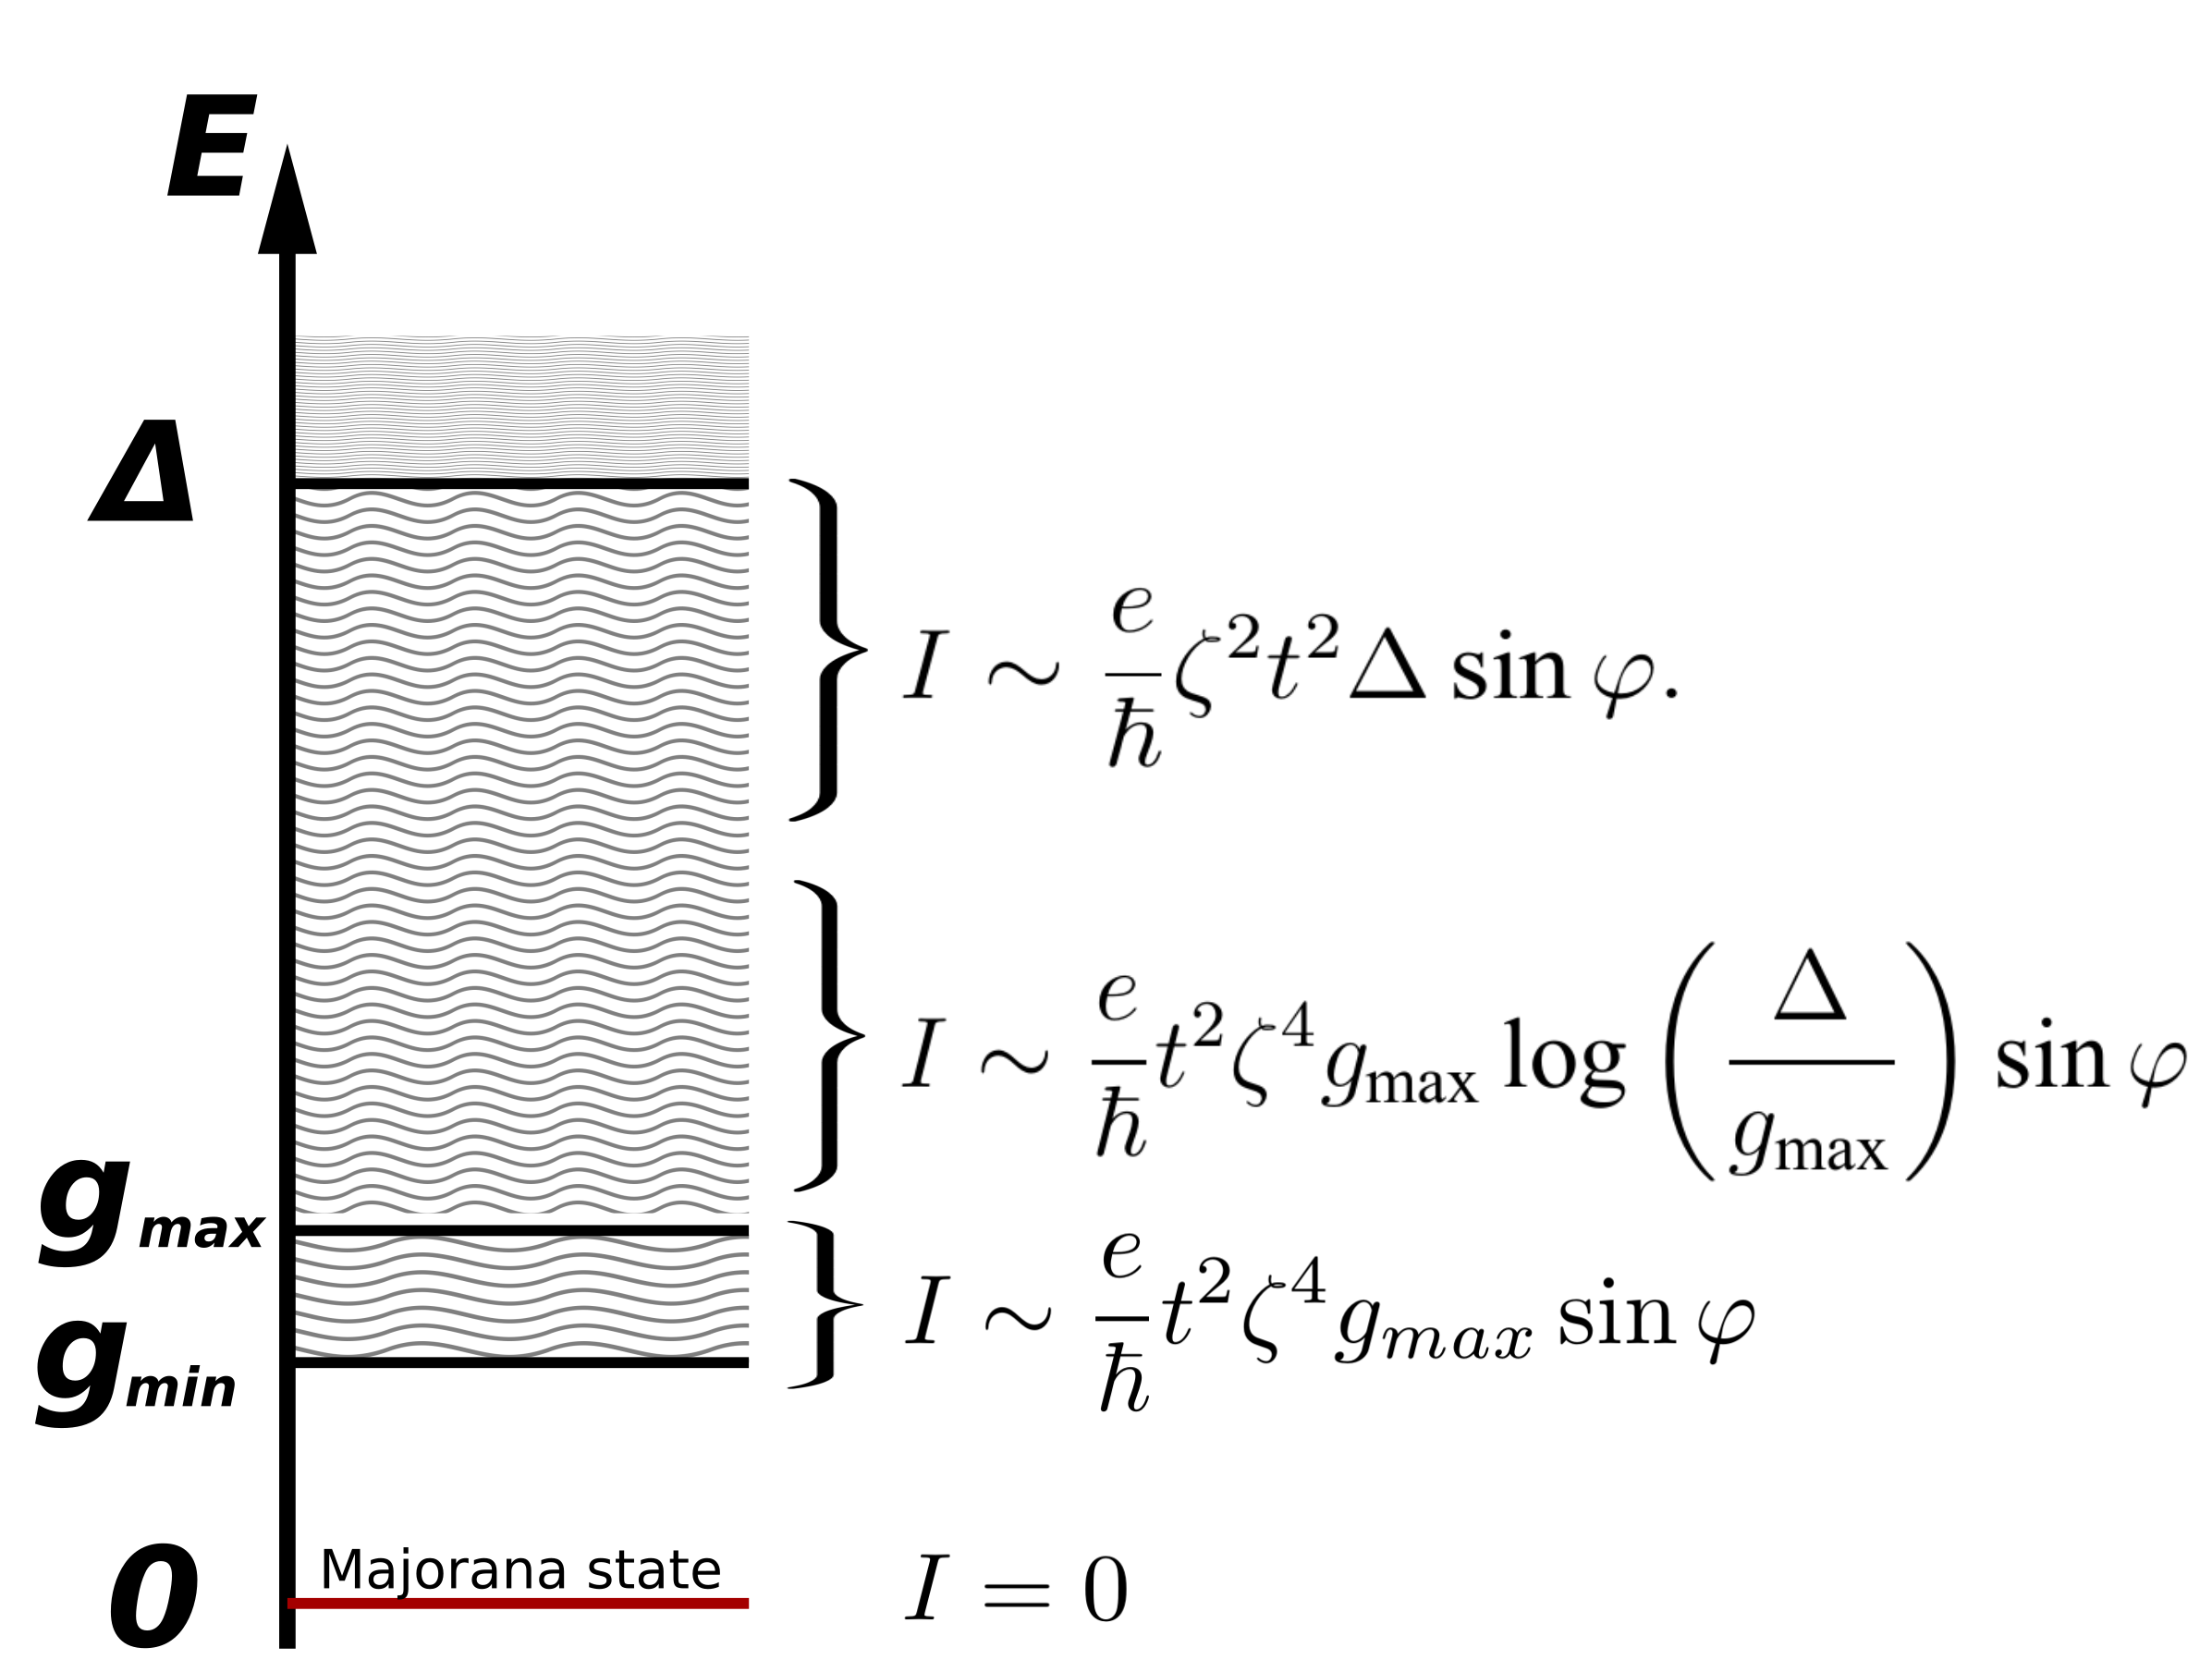
\includegraphics[width=0.7\linewidth]{images/supercurrent}
	\caption{Supercurrent from different states}
	\label{fig:supercurrent}
\end{figure}



 Thus we deduce that the current from the low energy states is negligible compared with the current from the states near $ \Delta. $ This shows us that the low energy states ($ E\ll\Delta $) contribute to stationary supercurrent by a very small quantity. The proportionality to $ \Delta $ in (\ref{curr_E_delta}) is similar to  a conventional Josephson tunnel junction. We conclude, that measuring stationary supercurrent is unlikely to reveal any topological physics in this system.


